\documentclass[11pt,a4paper]{article}
\usepackage[spanish,activeacute]{babel}
\decimalpoint
\usepackage[utf8]{inputenc}
\usepackage{listingsutf8}
\usepackage{amsmath}
\usepackage{amsfonts}
\usepackage{amssymb}
\usepackage{graphicx}
\usepackage{color}
\usepackage{listings}
\usepackage{amsthm}
\usepackage{caption}
\usepackage{subcaption}
\usepackage{dsfont}
\usepackage{comment}
\usepackage{enumerate}
\usepackage{mathtools,xparse}
\usepackage{ mathrsfs }
\usepackage{float}
\usepackage{listings}
\usepackage{xcolor}
\usepackage{esvect}
%% CODIGO PYTHON
\definecolor{codegreen}{rgb}{0,0.6,0}
\definecolor{codegray}{rgb}{0.5,0.5,0.5}
\definecolor{codepurple}{rgb}{0.58,0,0.82}
\definecolor{backcolour}{rgb}{0.93,0.93,0.93}

\lstdefinestyle{mystyle}{
    backgroundcolor=\color{backcolour},   
    commentstyle=\color{codegreen},
    keywordstyle=\color{magenta},
    numberstyle=\tiny\color{codegray},
    stringstyle=\color{codepurple},
    basicstyle=\ttfamily\footnotesize,
    breakatwhitespace=false,         
    breaklines=true,                 
    captionpos=b,                    
    keepspaces=true,                 
    numbers=left,                    
    numbersep=5pt,                  
    showspaces=false,                
    showstringspaces=false,
    showtabs=false,                  
    tabsize=2
}

\lstset{style=mystyle, inputencoding=utf8, extendedchars=true, literate={á}{{\'a}}1 {ó}{{\'o}}1 {é}{{\'e}}1 {ú}{{\'u}}1 {í}{{\'i}}1 {ñ}{{\~n}}1,}
%CODIGO PYTHON
\usepackage[left=2.33cm, right=2.31cm, top=2.42cm, bottom=2.42cm]{geometry}
%\renewcommand{\rmdefault}{mathpazo}
%\usepackage{mathpazo}

\usepackage[]{hyperref}
\hypersetup{
    pdftitle={Práctica 3 - AA},
    pdfauthor={Mario Muñoz Mesa},
    pdfsubject={ },
    pdfkeywords={keyword1, keyword2},
    bookmarksnumbered=true,     
    bookmarksopen=true,         
    bookmarksopenlevel=1,       
    colorlinks=true,   
    linkcolor=black,         
    pdfstartview=Fit,           
    pdfpagemode=UseOutlines,
    pdfpagelayout=TwoPageRight
}


\DeclarePairedDelimiter{\norm}{\lVert}{\rVert}
\NewDocumentCommand{\normL}{ s O{} m }{%
  \IfBooleanTF{#1}{\norm*{#3}}{\norm[#2]{#3}}_{L_2(\Omega)}%
}
\newtheorem{theorem}{Teorema}

\theoremstyle{definition}
\newtheorem{definition}{Definición}[section]


\newtheorem{proposition}{Proposición}[section]


\newtheorem{corolary}{Corolario}[section]


\newtheorem{lema}{Lema}[section]

	\newcommand{\R}{\mathbb{R}}
	\newcommand{\N}{\mathbb{N}}
	\newcommand{\C}{\mathbb{C}}


\title{
\normalfont \normalsize 
\textsc{\small APRENDIZAJE AUTOMÁTICO} \\ [10pt]
	
	
\huge \bf Práctica 3\\


	}

\author{Mario Muñoz Mesa}
\date{4 junio 2021}

\begin{document}

	\maketitle
	\renewcommand*\contentsname{Índice}	
	\tableofcontents
	
	\newpage
	
	\section{Regresión (Superconductivity)}
	\subsection{Planteamiento.}
	Suponemos $(\Omega, \mathcal{A}, P)$ espacio probabilístico, donde $\Omega$ es el conjunto de todos los posibles superconductores; $\mathcal{A}$ sigma-álgebra formada por todos los subconjuntos de $\Omega$, y $P$ distribución de probabilidad desconocida.
	
	Sobre $(\Omega, \mathcal{A}, P)$ tenemos el vector aleatorio $\mathbf{x}=(x_1,\ldots x_{81})$ donde cada variable aleatoria $x_i\colon \Omega \to \R$, $i\in \{1,\ldots,81\}$, mide: el número de elementos para $i=1$ y características relacionadas con: atomic mass, first ionization energy, atomic radius, density, electron affinity, fussion heat, thermal conductivity o valence, para $2\leq i \leq 81$. También tenemos la variable aleatoria $y\colon \Omega \to \R$ que asigna la temperatura crítica (grados Kelvin) a cada superconductor (más detalles en el documento adjunto a \href{https://archive.ics.uci.edu/ml/datasets/Superconductivty+Data}{
Superconductivity Data Set}). Por lo que $\mathcal{X}=\mathbf{x}(\Omega)=\R \times \stackrel{81}{\cdots} \times \R = \R^{81}$ y $\mathcal{Y}=y(\Omega)=\R$
	
	A partir del fichero alojado en \href{https://archive.ics.uci.edu/ml/datasets/Superconductivty+Data}{
Superconductivity Data Set} se toma $N < 21263$, que será el tamaño de la muestra de entrenamiento. Reservando el 20\% de los datos para test obtuvimos $N=17010 \iffalse- k\fi$%,

	En ambos casos, para conseguir estimación $g$ $\mathcal{H}$-lineal de $f$, y dado que tenemos muestra i.i.d., se seguirá el criterio ERM (minimización de riesgo empírico). Como tenemos que cuidar la cota de error de generalización, aplicaremos regularización para evitar sobreajuste.
	\iffalse
	Podemos obtener una representación 2D del conjunto de training sobre el que se trabajará mediante las 2 componentes principales 
	\begin{figure}[H]
		\centering
		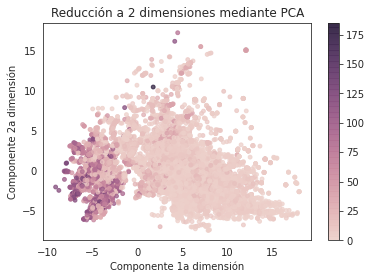
\includegraphics[width=0.6\textwidth]{images/repre_regre}
		\caption{Visualizamos reducción 2-dimensional de los vectores de características (realizada mediante PCA)}
	\end{figure}
	
	Podemos ver que con solo las 2 componentes principales no podríamos obtener ningún regresor lineal decente. Desde luego trabajaremos con bastantes más dimensiones.\fi
	\subsection{Clase de funciones a usar.}
	Realizaremos una transformación de segundo orden polinomial a los vectores de características, pues aumenta la flexibilidad de nuestra regresor. Para no aumentar en exceso la complejidad de la clase de funciones (mayor dimensión $\Rightarrow$ mayor complejidad $\Rightarrow$ mayor cota de error de generalización) reduciremos previamente la dimensionalidad de nuestros vectores de características (ver parte de preprocesado). No utilizamos transformación polinómica de mayor orden pues cuanto mayor sea la longitud de los vectores de características mayores posibilidades de disminuir el error en la muestra pero mayores posiblidades de aumentar error en la población (sobreajuste); a parte de incrementar el coste computacional.
	
	Por lo que, como hemos comentado, aplicaremos a  $\mathcal{X}$ la transformación $\Phi_2$, que genera combinaciones polinómicas de grado menor o igual que 2 de las características $$\Phi_2(\mathbf{x})=(1,x_1,\ldots, x_{\hat d},\underbrace{x_1x_2,\ldots ,x_1x_{\hat d},x_2x_3,\ldots ,x_2x_{\hat d},  \ldots
	 x_{\hat d-1}x_{\hat d}}_{\text{combinaciones } x_ix_j \text{ con } i<j,\ \  i,j\in \{1,\ldots , \hat d\}}, x_1^2,\ldots x_{\hat d}^2)^T$$
	%Realmente no podemos saber a priori cual es la mejor transformación que podemos hacer, debemos elegir una
	\textit{Nota:} aquí $\hat d< d=81$ pues no utilizaremos todas las características. Podemos ver que $\Phi_2(\mathbf{x})$ tiene $1+\hat d  + (\sum_{i=1}^{\hat d-1} \hat d -i) + \hat d  = 1 + 2\hat d + (\hat d -1)\hat d - \frac{(\hat d -1)\hat d}{2}=1+2\hat d + \frac{(\hat d -1)\hat d}{2}$ componentes\\
	
	Denotando con $d$ a $2\hat d + \frac{(\hat d -1)\hat d}{2}$, la clase de funciones hipótesis a usar será
	$$\mathcal{H}:=\{h_w\colon \R^{d+1} \to \R \ : \ h_w(\Phi_2(\mathbf{x}))=w^T\Phi_2(\mathbf{x}),\ w \in \R^{d+1}\}$$
	Denotando con $\mathbf{x}_i$ a $\Phi_2(\mathbf{x}_i)$, $i\in \{1,\ldots , N\}$, el error en la muestra a minimizar es
	$$E_{in} (w):=\frac{1}{N}\sum_{i=1}^N(w^T\mathbf{x}_i-y_i)^2$$
	es decir, la media del error cuadrático en cada uno de los elementos de la muestra. Equivalentemente, usando notación matricial
	$$E_{in}(w)=\frac{1}{N}\norm{Xw-y}^2$$
	donde
	$$
	X=\begin{matrix}
	& \left(\begin{matrix}
	- \mathbf{x}_1^T - \\
	- \mathbf{x}_2^T - \\
	...  \\
	- \mathbf{x}_N^T - \\


	\end{matrix}\right)
	\end{matrix}
		\quad \quad 
	y=\begin{matrix}
	& \left(\begin{matrix}
	y_1 \\
	y_2 \\
	...  \\
	y_N  \\


	\end{matrix}\right)
	\end{matrix}
	$$
	
	Queremos minimizar
	$$E_{in}(w)=\frac{1}{N}\norm{Xw-y}^2=\frac{1}{N}(Xw-y)^T(Xw-y)=\frac{1}{N}((Xw)^TXw-y^TXw-(Xw)^Ty+y^Ty1)=$$ $$=\frac{1}{N} (w^TX^TXw-2w^TX^Ty+y^Ty)$$
	es decir, buscamos vector de pesos $\hat w \in \R^{d+1}$ con $E_{in}(\hat w)=\min_{w\in \R^{d+1}} E_{in}(w)$. El gradiente queda 
	$$\nabla E_{in}(w)=\frac{2}{N} X^T (Xw-y)=2X^TXw-2X^Ty$$ ~\\
	
	Técnicas conocidas para obtener mínimo de $E_{in}$ en regresión lineal:\\
	
	\textbf{Gradiente Descendente:} $\quad \quad \quad \quad \quad \quad \quad \quad \quad \quad \quad \quad \quad \quad \quad \quad \quad \quad \quad \quad \quad  $ %(\texttt{SGDRegressor})
	
	\textit{Gradiente Descendiente} es una técnica general para obtener mínimos de una función derivable. Una analogía ilustrativa es una bola rodando por una superficie con colinas. Si la bola se emplaza en la colina, esta desciende hasta encontrar un valle (mínimo local). Igual ocurre con $E_{in}(w)$, que se puede representar como una superficie de altas dimensiones.
	
	 En el comienzo del algoritmo empezamos en un punto $w_0$ del dominio de $E_{in}$.
	
	%\textit{Nota:}  en el caso de $E_{in}(w)$ solo tiene un bajada por ser convexa, no hay mínimo locales solo uno global (el estudio se hará en general).
	
	Tenemos que determinar cómo bajar por $E_{in}$ mediante ``el paso más profundo''. Supongamos que tomamos un paso de tamaño $\eta$ (tasa de aprendizaje) en la dirección de un vector unitario $\hat v$, $\norm{\hat v}=1$. El nuevo valor del dominio de $E_{in}$ a utilizar será $w_0+\eta \hat v$. Queremos, dado $w_0$, encontrar $\hat v$ tal que $$E_{in}(w_0+\eta \hat v)<E_{in}(w_0)$$
Se toma $\eta$ pequeño, $\eta \approx 0$. Aplicaremos desarrollo de Taylor en la siguiente expresión
	$$\Delta E_{in}=E_{in}(w_0+\eta \hat v) - E_{in}(w_0)\stackrel{Taylor}{=} \eta \nabla E_{in}(w_0)^T\hat v + \underbrace{\mathcal{O}(\eta ^2)}_{\text{O-grande}} \geq  \eta \nabla E_{in}(w_0)^T\hat v  \stackrel{(*)}{=}$$ $$ \stackrel{(*)}{=}-\eta \norm{\nabla E_{in}(w_0)}$$
	(*) En la última igualdad tenemos el producto del vector fila $\eta \nabla E_{in}(w_0)^T$ (que es evaluar $w_0$ en el gradiente de $E_{in}$ como fila), y por otro lado el vector que yo quisiera elegir $\hat v$. Para que este producto escalar sea máximo $\hat v$ debe tener misma dirección y sentido que $\eta \nabla E_{in}(w_0)^T$, así el coseno del ángulo que forman será 1. Pero como lo que nosotros buscamos es minimizar, tomaremos sentido opuesto para que el producto sea negativo (notar de nuevo que buscamos $E_{in}(w_0+\eta \hat v)<E_{in}(w_0)$). Entonces $\eta \nabla E_{in}(w_0)^T$ y $\hat v$ coinciden en la misma dirección pero con sentidos opuestos, es decir, $\hat v$ tiene la dirección y sentido de $-\nabla E_{in}(w_0)$. Finalmente, basta hacer el producto escalar de $\eta \nabla E_{in}(w_0)^T$ y $\hat v$  para ver la igualdad $$\eta \nabla E_{in}(w_0)^T \hat v\stackrel{(*)}{=} \eta \norm{\nabla E_{in}(w_0)^T} \norm{\hat v} \cos(\pi)=-\eta \norm{\nabla E_{in}(w_0)} $$
	$$\Leftrightarrow \nabla E_{in}(w_0)^T \hat v= -\norm{\nabla E_{in}(w_0)} \Leftrightarrow \frac{\nabla E_{in}(w_0)^T \hat v}{\norm{\nabla E_{in}(w_0)}}= -1 \Leftrightarrow \hat v=-\frac{\nabla E_{in}(w_0)}{\norm{\nabla E_{in}(w_0)}}$$
	Por tanto
	$$\hat v=-\frac{\nabla E_{in}(w_0)}{\norm{\nabla E_{in}(w_0)}}$$
	
	Una vez que está definido el vector que usaremos para desplazarnos en busca de un mínimo, podemos describir el proceder del algoritmo. Se toma una tasa de aprendizaje $\eta$, un punto inicial $w=w_0\in \text{Dominio}(E_{in})$, y se actualiza el valor de $w$ repetidamente
	$$w:=w-\eta \nabla E_{in}(w)$$
	repetimos esta actualización hasta una condición de parada, ya sea por iteraciones o por encontrar un valor suficientemente pequeño.\\
	
	\textbf{Gradiente Descendente Estocástico:}
	
	Este método, a diferencia de \textit{Gradiente Descendente}, trabaja con minibatches (pequeñas submuestras de la muestra). Está comprobado empíricamente que el uso de estos minibatches para el cálculo del gradiente mejora el óptimo obtenido para funciones no convexas. Al trabajar con submuestra pequeña es probable que en los pasos o desplazamientos del algoritmo se evite caer en mínimos locales no deseables (valor alto), mínimos locales en los que sí se entraría si trabajasemos con toda la muestra.

	\iffalse Una vez que está definido el vector que usaremos para desplazarnos en busca de un mínimo, podemos describir el proceder del algoritmo.\fi Se toma una tasa de aprendizaje $\eta$, un punto inicial $w=w_0\in \text{Dominio}(E_{in})$. Se divide la muestra en una secuencia de minibatches aleatorios. Iteramos los minibatches y en base a cada minibatch, $minibatch \in Minibatches$, se actualiza el valor de $w$
	$$w:=w-\eta \nabla E_{in}^{minibatch}(w)$$
	repetimos esta división en minibatches y los cálculos de $w$ por cada $minibatch \in Minibatches$ \iffalse esta toma de minibatch y cálculo de $w$ en función del minibatch\fi hasta una condición de parada, ya sea por iteraciones o por encontrar un valor suficientemente pequeño para $E_{in}$\\
	
	\textbf{Pseudoinversa (solución analítica):} $\quad \quad \quad \quad \quad \quad \quad \quad \quad \quad \quad \quad \quad \quad \quad \quad \quad \quad \quad \quad \quad \quad \quad \quad \quad \quad \quad \quad  \quad $ %(\texttt{Ridge})
	
    Mediante este método obtenemos analíticamente la solución óptima. Para minimizar $E_{in}$ igualamos gradiente a 0
	$$\nabla E_{in}(w)=\frac{2}{N} X^T (Xw-y)=2X^TXw-2X^Ty=0$$
	y queda
	$$X^TXw= X^Ty$$
	que se reescribe como
	$$w=X^\dagger y \quad \text{ donde } \quad X^\dagger :=(X^TX)^{-1}X^T \ \ \text{ (pseudo-inversa de } X\text{)}$$
	$\Rightarrow w_{lin}=X^\dagger y$.
	Por tanto, dados $X$ e $y$, el algoritmo consiste en calcular $X^\dagger =(X^TX)^{-1}X^T$ y devolver $w_{lin}=X^\dagger y$
	
	Para calcular $(X^TX)^{-1}$ se puede usar la descomposición en valores singulares (SVD), $X=UDV^T$, y queda $(X^TX)^{-1}=VD^*V^T$ (si $D$ tiene $e_0,\ldots,e_d$ como elementos de la diagonal, la matriz $D^*$ tiene, en la diagonal, $\frac{1}{e_i^2}$ como elementos o $0$ si $e_i=0$) \\
	
	\textit{Nota:} Una desventaja de este método es que el cálculo matricial hace que no sea un método con buena escalabilidad, grandes cantidades de datos pueden dar lugar a matrices no abordables.
	

	\subsection{Hipótesis finales que se usarán.}
	En el preprocesado: (1) se eliminan características con coeficiente de correlación lineal en valor absoluto mayor a 0.95, (2) se eliminan las características con varianza 0, (3) se seleccionan las combinaciones de características mediante PCA que expliquen al menos el 97\% de la varianza (4) se realiza transformación polinomial de segundo orden a cada vector de características, (5) se normalizan las características (media 0 y varianza 1).
	
	La métrica a valorar es ECM. Evaluaremos desempeño de los métodos \texttt{SGDRegressor} (Gradiente Descendente Estocástico), \texttt{Ridge} (sol analítica SVD) (regularización $l_2$ en ambos) y \texttt{Lasso} (descenso de coordenadas) (regularización $l_1$), para cada uno evaluaremos los parámetros de regularización $0.00001$, $0.001$ y $0.1$ mediante 5-fold cross validation
	\subsection{Generación de conjuntos training y test.}
	Hay un compromiso en la selección del tamaño de entrenamiento y test: el tamaño de la muestra de entrenamiento determina el número de instancias que tendremos para entrenar el modelo y por tanto para minimizar $E_{in}$, y el  tamaño del conjunto de test condicionará la estimación, $E_{test}$, de $E_{out}$ que obtengamos. Evitaremos proporciones extremas de tamaño para test. Suele ser habitual reservar un 20\% de las instancias para test, y eso hemos hecho. De las 21263 instancias tendremos 17010 para test, el resto para training y validación cruzada.
	
	Utilizaremos $k$-fold cross validation con $k=5$ para la selección de modelos. Esta técnica es derivada de \textit{Leave-one-out}, la cual nos proporciona una estrategia para abordar la problemática o compromiso de elección del tamaño de conjunto de validación, $K$, esta es: $E_{out}(g)\approx E_{out}(g^-)$ cuando $K$ pequeño y $E_{out}(g^-)\approx E_{val}(g^-)$ cuando $K$ grande. %Lo ideal sería utilizar $N$-fold cross validation que equivale a \textit{Leave-one-out}, pero tiene un alto coste computacional.
	
	 La técnica $k$-fold cross validation consiste en dividir la muestra de entrenamiento en $k$ particiones, cada una de tamaño aproximado $\frac{N}{k}$, e ir iterando sobre ellas eligiendo cada vez una partición para actuar como conjunto de validación y entrenando sobre el resto de la muestra el modelo; una vez iteradas sobre todas las particiones se toma la media de errores obtenidos y ese es el error de validación cruzada $E_{cv}\iffalse=\frac{1}{N}\sum_{i=1}^N E_{val}(g_i^-)\fi$ que es un buen estimador de $E_{out}$ cuando $k$ es grande, cuanto menor sea $k$ peor será la estimación de $E_{out}$. Se elige el modelo con menor $E_{cv}$
	 
	  Se podría tomar $k=N$ (Leave-one-Out) pero esto implica un alto coste computacional; es por esto que se elige $k<< N$, en nuestro caso $k=5$ (es habitual $5\leq k\leq 10$)
	\subsection{Detalles del preprocesado de datos.}
	Pasos realizados:
	\begin{enumerate}
		\item Se eliminan las características que tienen valor absoluto de coeficiente de correlación lineal mayor a 0.95 con otra característica. %Se puede decir que éstas no nos aportan información nueva.
		
		Esto se hace porque se observó la matriz de coeficientes de correlación en valores absolutos
		\begin{figure}[H]
		\centering
		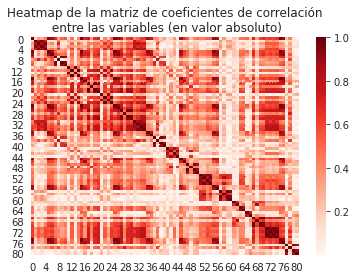
\includegraphics[width=0.5\textwidth]{images/corr_matrix_regre}
		\caption{Matriz de coeficientes de correlación en valor absoluto}
		\end{figure}
		Las características $4, 9, 13, 14, 15, 19, 24, 25, 26, 29, 30, 34, 39, 49, 54, 59, 69, 70, 73, 74, 75, 76, 79$ tenían valores de coeficiente de correlación lineal mayor a 0.95 en la matriz. Se puede decir que estas características no nos aportan información nueva, además aumentan la dimensionalidad y por tanto empeoran la cota de error de generalización. Se decide eliminarlas y reducir así la complejidad de la clase de funciones. Tras eliminarlas se obtiene
		\begin{figure}[H]
		\centering
		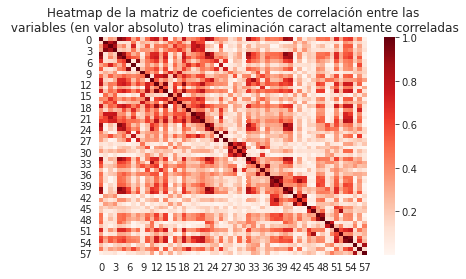
\includegraphics[width=0.62\textwidth]{images/corr_matrix_post_regre}
		\caption{Matriz de coeficientes de correlación en valor absoluto tras la eliminación de características altamente correladas linealmente}
		\end{figure}
		una matriz de menor dimensión y con menor apreciación de zonas correspondientes a alta correlación (excepto en diagonal donde tenemos coeficientes de correlación 1 pues es la correlación de cada característica consigo misma).
		\item Eliminamos las características con varianza 0 si las hubiese, no aportan ninguna información y además es necesario eliminarlas para después normalizar.
		\item Normalizamos las características (media 0 y varianza 1) para el correcto funcionamiento de PCA
		%\item Normalizamos las características, no normalizarlas degrada el desempeño de la regularización.
		%\item Una vez normalizadas y teniendo ????
		\item Seleccionamos las combinaciones de características mediante PCA que expliquen al menos el 97\% de la varianza. Mediante este método esperamos reducir la dimensionalidad con la mayor información posible; de modo que cuando apliquemos la transformación polinómica no tengamos una dimensionalidad excesiva (dimensionalidad muy alta aumenta coste computacional y mayor cota de error de generalización).
		La elección de este método ha sido arbitraria, se podría haber elegido cualquier otro método para reducir reducir la dimensionalidad y complejidad de la clase de funciones.
		\item Realizamos transformación polinomial de segundo orden a cada característica para aumentar así la flexibilidad de nuestro regresor.
		\item Normalizamos las características (tendrán media 0 y varianza 1), no normalizar puede degradar el desempeño de métodos como Lasso y SGD por ejemplo. También deben estar normalizadas de cara a que nuestra regularización actúe correctamente. Normalizamos para evitar estas problemáticas y que todas las características ``sean valoradas en la misma magnitud''.
		\end{enumerate}
	\subsection{Métrica de error a usar.}
	La métrica que utilizaremos es el error cuadrático medio, ECM, $ECM= \frac{1}{N} \sum_{i=1}^N (h_w(x_i)-y_i)^2$ que nos da la media de la suma de los errores cuadráticos de las diferencias entre las predicciones y las verdaderas etiquetas. Tiene como desventaja que no está acotada superiormente y no tenemos por tanto una referencia de cuánto de malo es un resultado en concreto. Aún así es de uso extendido, es la misma función que se minimiza, y nos servirá para comparar los modelos.
	
	Otra métrica conocida consiste en tomar valor absoluto en la diferencia entre predicciones y verdaderas etiquetas en vez de elevar al cuadrado la diferencia. En este caso tendríamos la media de los valores absolutos de las diferencias (Error Medio Absoluto), sin embargo no consideramos que sea de interés pues usándola daríamos menos importancia a los errores altos que con ECM.
	\subsection{Parámetros usados y tipo de regularización elegida.}
	La regularización nos ayudará a evitar sobreajuste, sobretodo después de la transformación polinómica que hemos realizado. Con la regularización se aumentará ligeramente el sesgo para decrementar significativamente la varianza.
	
	Tenemos cierta confianza en haber eliminado características redundantes en el preprocesado. Una hipótesis será asumir que esto ha ocurrido y que la mayoría de nuestras características son informativas y tienen un impacto en el etiquetado. Bajo esta hipótesis utilizaremos dos modelos con regularización Ridge, por lo que tendremos en ellos error aumentado
	$$E_{aug}(\mathbf{w})=E_{in}(\mathbf{w})+\lambda \norm{\mathbf{w}}_2^2 = E_{in}(\mathbf{w})+\lambda \mathbf{w}^T\mathbf{w}$$
	donde $\lambda \geq 0$ es el parámetro de regularización (este tipo de regularización penaliza los coeficientes de $\mathbf{w}$ grandes).  
	
	Por otra parte, estamos trabajando en un problema con bastantes características y de diversa índole (varias caract. sobre radio atómico, varias sobre temperatura de fusión...), y mediante PCA reducimos dimensionalidad teniendo solo en cuenta las características y no el etiquetado. %, lo que motiva utilizar un modelo con regularización Lasso y comprobar su desempeño (regularización Lasso suele funcionar bien cuando hay bastantes caract. poco informativas y regularización Ridge cuando son pocas las características poco informativas).
	La otra hipótesis será que aún queda un número significativo de características redundantes. Bajo esta hipótesis utilizaremos un modelo con regularización Lasso (regularización Lasso suele funcionar bien cuando hay bastantes caract. poco informativas y regularización Ridge cuando son pocas las características poco informativas), por lo que tendremos error aumentado 
	$$E_{aug}(\mathbf{w})=E_{in}(\mathbf{w})+\lambda \norm{\mathbf{w}}_1$$
	donde $\lambda \geq 0$ es el parámetro de regularización. Con regularización Lasso penalizaremos las características poco informativas (cuando se minimiza con este tipo de regularización tiende a poner coeficientes de $\mathbf{w}$ a 0 en las características poco informativas), si hubiese un número significativo de caract. redundantes esperamos obtener mejor resultado que con regularización Ridge. \\
	
	Para técnica Gradiente Descendente Estocástico se utiliza la función \texttt{SGDRegressor}. Ésta utiliza tamaño minibatch 1. Es interesante notar que la función de error junto con el término de regularización Ridge es convexa; pierde relevancia el uso de minibatches o punto de inicio al no tener óptimos locales. Se podría utilizar Gradiente Descendente sin ningún problema. Aún así, dado que \texttt{sklearn} nos proporciona método para la versión estocástica, y que realmente ganamos eficiencia computacional al calcular gradiente en un solo punto, y el ruido que supone computar el gradiente en un solo punto termina promediándose en número alto de iteraciones; se decide utilizar la versión que nos facilita \texttt{sklearn}. El learning rate se ha elegido adaptativo, cuando no se esté mejorando en el criterio de tolerancia tras \texttt{n\_iter\_no\_change} épocas, entonces actualizamos la tasa de aprendizaje mediante $learning\_rate =\frac{learning\_rate}{5}$, vamos disminuyendo conforme nos acercamos al mínimo para evitar oscilación. Elegimos \texttt{n\_iter\_no\_change}=1 y una tolerancia \texttt{tol} muy baja; si tras una época no hemos conseguido reducir una cantidad ínfima el error, entonces estaremos oscilando por learning rate muy alto, y por tanto se decrementará. El algoritmo parará cuando si llegamos a learning rate 1e-6 o por iteraciones máximas. Se adjunta código con comentarios del resto de parámetros:% Es interesante notar que la función de error junto con el término de regularización Ridge es convexa, pierde relevancia el uso de minibatches o punto de inicio al no tener óptimos locales. Se adjunta código con comentarios del resto de parámetros:
	\begin{lstlisting}[language=Python, caption= Par\'ametros usados en \texttt{SGDRegressor}, inputencoding=latin1]
  {"model": [SGDRegressor(loss = 'squared_loss', # función de pérdida cuadrática
                                 penalty = 'l2', # utilizaremos regularización l2
                                 # alpha  constante del término de regularización (probaremos distintos valores mediante 5-fold cross validation)
                                 fit_intercept = True, # añadimos sesgo o intercept pues nuestra matriz aún no tiene columna de 1s 
                                 max_iter = 4100, # Número máximo de iteraciones arbitrario
                                 tol = 0.000001, # Tolerancia para criterio de parada por tolerancia (parar si loss > best_loss - tol tras n_iter_no_change épocas seguidas)
                                             # el criterio valora si el error es no mejora en 0.001 el mejor error hasta el momento. En nuestro caso esta condición por tolerancia se usará para learning_rate adaptativo
                                 shuffle = False, # no nos interesa introducir más ruido
                                 random_state = 1, # para tener reproducibilidad de los resultados
                                 learning_rate = 'adaptive', # si no se mejora resultado por criterio tolerancia (loss > best_loss - tol) tras n_iter_no_change épocas seguidas, entonces cambiamos learning rate por (learning rate)/5
                                                             # queremos evitar oscilación
                                 eta0 = 0.05, # learning rate inicial arbitrario, nos permitimos que sea un poco alto pues es adaptativo
                                 early_stopping = False, # False pues no queremos reservar más datos para validación
                                 n_iter_no_change = 1, # cada época sin mejora en crit. tolerancia se realizará la adaptación del learning rate (learning_rate='adaptive')
                                 average = False, # no nos interesa obtener media de pesos
                                 verbose = 0, # no nos interesan mensajes 
                                 warm_start = False, # no reutilizamos ninguna solución anterior durante la validación cruzada
                                 l1_ratio = 0 # 0 corresponde a l2 penalty, no se usará pues solo se usa si learning_rate = 'elasticnet'
                                 )],
         "model__alpha": [0.00001, 0.001, 0.1]}, # probamos valores de regularización arbitrarios dentro de los recomendados

	\end{lstlisting}
	Otro de nuestros modelos consiste en obtener una solución analítica mediante descomposición en valores singulares, para ello se utiliza la función \texttt{Ridge} indicando método de resolución ``svd'' que nos dará la solución solución óptima de la función de error con regularización Ridge (error aumentado) haciendo uso de la descomposición en valores singulares de $X$. Se adjunta código con comentarios sobre los parámetros elegidos:
	\begin{lstlisting}[language=Python, caption= Par\'ametros usados en \texttt{Ridge}, inputencoding=latin1]
  {"model": [Ridge(# alpha  constante del término de regularización (probaremos distintos valores mediante 5-fold cross validation)
                         fit_intercept = True, # añadimos sesgo o intercept pues nuestra matriz aún no tiene columna de 1s
                         normalize = False, # ya hemos normalizado en preprocesado
                         copy_X = True, # no nos interesa sobreescribir X
                         max_iter = None, # pues resolveremos mediante método analítico
                         # tol lo podemos dejar por defecto pues no se va a usar
                         solver = 'svd', # resolveremos de forma analítica usando descomposición en valores singulares 
                         random_state=None)], # no nos hace falta para tener reproducibilidad de los resultados pues no se va a usar solver=sag o solver=saga. Obtendremos solución analítica
         "model__alpha": [0.00001, 0.001, 0.1]}, # probamos valores de regularización arbitrarios dentro de los recomendados

	\end{lstlisting}
	\textit{Nota:} sabemos que, permitiéndolo el tamaño del dataset, mediante un método analítico siempre obtendremos la solución óptima mientras que por Gradiente Descendente Estocástico obtendremos una estimación del mínimo. Aún así, para el propósito de la práctica, mantenemos el de Gradiente Descendente Estocástico, utilizaremos ambos y así también comprobaremos lo comentado.\\
	
	Por último, para nuestro modelo con regularización Lasso, utilizamos la función \texttt{Lasso}, que utiliza algoritmo de descenso de coordenadas en lugar de Gradiente Descendente Estocástico (va actualizando un parámetro cada vez en lugar de todos como en Gradiente Descendente Estocástico). Adjuntamos código con los parámetros comentados:
	\begin{lstlisting}[language=Python, caption= Par\'ametros usados en \texttt{Lasso}, inputencoding=latin1]
  {"model": [Lasso(# alpha  constante del término de regularización (probaremos distintos valores mediante 5-fold cross validation)
                         fit_intercept = True, # añadimos sesgo o intercept pues nuestra matriz aún no tiene columna de 1s
                         normalize = False, # ya hemos normalizado en preprocesado
                         precompute = False, # tampoco tenemos demasiados datos
                         copy_X = True, # no nos interesa sobreescribir X
                         max_iter = 3000, # número máximo de iteraciones arbitrario
                         tol = 0.0001, # el por defecto, parece una tolerancia razonable. Elección arbitraria
                         warm_start = False, # no reutilizamos soluciones anteriores como inicio
                         positive = False, # no tenemos necesidad de que los coef. sean positivos
                         random_state = 1, # para tener reproducibilidad de los resultados
                         selection = 'cyclic')], # no tenemos tol > 1e^-4 para que pueda resultar interesante 'random'
         "model__alpha": [0.00001, 0.001, 0.1]}, # probamos valores de regularización arbitrarios dentro de los recomendados 

	\end{lstlisting} ~\\
	
	\textit{Nota en general:} el número de iteraciones, \texttt{n\_iter\_no\_change} y tolerancia se han elegido de forma arbitraria y comprobando que hubiese convergencia. Estos parámetros se podrían haber añadido como parámetros a valorar y expandir nuestro número de modelos para validación cruzada, pero los tiempos de ejecución serían inabarcables.
	
	\subsection{Selección de la mejor hipótesis y $E_{out}$}
	Para la selección de la mejor hipótesis o modelo utilizaremos 5-fold cross validation, técnica ya explicada en la sección de \textit{Generación de conjuntos training y test}. Elegiremos como modelo ganador aquel con menor $E_{cv}$. El modelo ganador se entrenará finalmente sobre toda la muestra.
	
	Para hacer esto se ha utilizado \texttt{GridSearchCV}, función que nos permite entrenar el modelo ganador en toda muestra mediante \texttt{refit=True}, y nos facilita variables con los resultados obtenidos. La métrica considerada para elección del mejor modelo es ECM (error cuadrático medio)
	
	Vamos a valorar distintos parámetros de regularización: tanto para \texttt{SGDRegressor}, \texttt{Ridge} y \texttt{Lasso} tendremos los parámetros de regularización $0.00001$, $0.001$ y $0.1$, por lo que en total tendremos 9 modelos para 5-fold cross validation (se podrían tener más modelos considerando otros parámetros, nos hemos limitado a los parámetros de regularización indicados)
	
	Nos referiremos a los modelos o hipótesis finalmente determinados por \texttt{SGDRegressor}, \texttt{Ridge} y \texttt{Lasso} (junto sus parámetros) mediante $M_{SGDRegressor}$, $M_{Ridge}$ y $M_{Lasso}$ (representan todos los pasos realizados: preprocesado, clase de funciones elegida, parámetros...). Tendremos 9 modelos determinados finalmente por los parámetros de regularización: $$\{(M_{SGDRegressor},\lambda),(M_{Ridge},\lambda),(M_{Lasso},\lambda)\} \ \ \text{ con } \ \ \lambda \in \{0.00001, 0.001, 0.1\}$$
	
	Veamos los ECM medios de cada modelo obtenidos por 5-fold cross validation
	%$(M_{PLA-Pocket},0.00001),\\ (M_{PLA-Pocket},0.0001), (M_{PLA-Pocket},0.1), (M_{RL},0.00001), (M_{RL},0.0001), (M_{RL},0.1)$
	\begin{table}[H]
	\begin{center}
	\begin{tabular}{|c|c|c|}
	\hline
	 Modelo & ECM medio 5-fold cross validation ($E_{cv}$) \\
	\hline \hline
	$(M_{SGDRegressor},0.00001)$ & 266.01612282 \\ \hline
	$(M_{SGDRegressor},0.001)$ & 262.30992773 \\ \hline
	$(M_{SGDRegressor},0.1)$ & 297.55736393 \\ \hline
	$(M_{Ridge},0.00001)$ & 261.96442557 \\ \hline
	$(M_{Ridge},0.001)$ & 261.96439522 \\ \hline
	$(M_{Ridge},0.1)$ & 261.96137422 \\ \hline
	$(M_{Lasso},0.00001)$ & 261.96321889 \\ \hline
	$(M_{Lasso},0.001)$ & 261.85022276\\ \hline
	$(M_{Lasso},0.1)$ & 270.32063746 \\ \hline
	\end{tabular}
	\caption{ECM medios por 5-fold cross validation de cada modelo}
	\label{tabla:sencilla}
	\end{center}
	\end{table}
	Nuestro mejor modelo con ECM por 5-fold cross validation 261.85022276 es $(M_{Lasso},0.001)$. En $M_{SGDRegressor}$ vemos buen resultado en ECM con un valor intermedio de regularización, poca regularización no da buen resultado. Y al aumentar valores de $\lambda$ estamos imponiendo restricción cada vez más fuerte y el modelo deja de ajustar bien como podemos observar, para $(M_{SGDRegressor},\lambda)$ con $\lambda=0.1$ obtenemos ECM 297.55736393, bastante peor.
	
	 En $M_{Ridge}$ podemos observar las soluciones óptimas para regularización Ridge, es destacable que el ECM no aumenta conforme incrementamos el valor de regularización, es más, el mejor resultado lo obtenemos con el mayor parámetro de regularización, $\lambda = 0.1$. Esto puede sugerir que en \texttt{SGDRegressor}, al modificar la función de error a minimizar (por aumentar $\lambda$) los parámetros dejan de ser adecuados y no llegamos a las soluciones óptimas.
	
	Finalmente, en $M_{Lasso}$ vemos que obtenemos la mejor solución con el valor intermedio de los parámetros de regularización, $\lambda = 0.001$. Con Lasso obtenemos una buena solución, de hecho la mejor en nuestra validación cruzada, lo cual podría sugerir que sí había características redundantes, aunque es difícil concluir nada pues nuestro grid es algo limitado y la diferencia de ECM con los modelos $M_{Ridge}$ es bastante baja. \\
	
	Entrenamos nuestro modelo ganador $(M_{Lasso},0.001)$ con todos los datos de entrenamiento. Al utilizar todos los datos de entrenamiento tenemos la ventaja de tener un tamaño de entrenamiento mayor (en 5-fold cross validation no utilizábamos $N$ instancias, siempre reservábamos una de las 5 particiones para validar). Entrenando sobre toda la muestra de entrenamiento se espera ahora obtener un ``mejor regresor''.
	
	 Utilizaremos nuestro conjunto de test que guardamos desde el principio para estimar el error de generalización, estimaremos $E_{out}$ mediante $E_{test}$. Procediendo así, estimamos, de nuestro mejor modelo $(M_{Lasso},0.001)$, ECM 261.58582397 fuera de la muestra; estimación ligeramente más optimista que la que obteníamos en validación cruzada (261.85022276), lo cual va en consonancia con el resultado teórico $E_{out}(g) \leq E_{cv}$ (va en consonancia en el sentido de que $E_{out}(g)\approx E_{test}(g)\leq E_{cv}$), que nos viene a decir que el error de validación cruzada, $E_{cv}$, nos da una estimación pesimista del error de generalización.
	
	\subsection{$E_{out}$ para la mejor hipótesis usando todos los datos para entrenar.}
	Ahora utilizamos todos los datos disponibles para entrenar nuestro mejor modelo, esto nos dará un mejor ajuste. Para estimar $E_{out}$ ya no disponemos de conjunto de test. Lo que se hará es hacer uso de la cota pesimista de que nos proporciona $E_{cv}$, tendremos una cota superior de $E_{out}(g)$. La cota será más ajustada cuanto mayor sea $k$ en $k$-fold cross validation, idealmente $k=N$ (Leave-one-out); de nuevo, por el alto coste computacional que esto supondría, nos conformaremos con $k=20$\\
	Procediendo así, estimamos $E_{out}(g)\leq 259.9156633155395$. Al estar usando todos los datos disponibles para entrenar estamos obteniendo un ``mejor regresor'', obtenemos como cota pesimista de $E_{out}$ un valor menor que la estimación que teníamos de $E_{out}$ por $E_{test}$ cuando solo usábamos el conjunto de training para entrenar (que a su vez era menor que el error de validación cruzada).
	%Al utilizar todos los datos de entrenamiento tenemos la ventaja de tener un tamaño de entrenamiento mayor (en 5-fold cross validation no utilizábamos $N$ instancias, siempre reservábamos una de las 5 particiones para validar). Entrenando sobre toda la muestra de entrenamiento se espera ahora obtener un ``mejor regresor''.
	
	%En este caso, para estimar $E_{out}$ utilizaremos el conjunto de test que guardamos desde el principio, calcularemos $E_{test}$. Procediendo así, estimamos ECM 261.58582397 fuera de la muestra, estimación ligeramente más optimista que la que obteníamos en validación cruzada (va en concordancia la desigualdad anteriormente mencionada $E_{out}(g) \leq E_{cv}$).
	
	%$E_{out}$ no se puede conocer solo estimar. Recordamos que el error $E_{cv}$  es buen estimador de $E_{out}$ ($E_{cv}$ es estimador insesgado de $\overline{E}_{out}(N-1)$; además $E_{out}(g) \leq E_{cv}$\iffalse , aunque trabajaremos con estimaciones y nos limitamos a unos datos, no siempre se tiene que cumplir\fi ). Estimamos ECM, de nuestro mejor modelo, $(M_{Lasso},0.001)$, fuera de la muestra 261.85022276
	\newpage
	
	\section{Clasificación (Sensorless Drive Diagnosis)}
	\subsection{Planteamiento.}
	Suponemos $(\Omega, \mathcal{A}, P)$ espacio probabilístico, donde $\Omega$ es el conjunto de posibles configuraciones, de componentes intactas y defectuosas, de motor; $\mathcal{A}$ sigma-álgebra formada por todos los subconjuntos de $\Omega$, y $P$ distribución de probabilidad desconocida.
	
	Sobre $(\Omega, \mathcal{A}, P)$ tenemos el vector aleatorio $\mathbf{x}=(x_1,\ldots x_{48})$ donde cada variable aleatoria $x_i\colon \Omega \to \R$, $i\in \{1,\ldots,48\}$, mide una señal eléctrica del dispositivo (rango $\R$ pues no se nos especifica ninguna cota), y la variable aleatoria $y\colon \Omega \to \{1,\ldots, 11\}$ que clasifica el estado del motor. Por lo que $\mathcal{X}=\mathbf{x}(\Omega)=\R \times \stackrel{48}{\cdots} \times \R = \R^{48}$ y $\mathcal{Y}=y(\Omega)=\{1,\ldots,11\}$
	
	A partir del fichero alojado en \href{https://archive.ics.uci.edu/ml/datasets/Dataset+for+Sensorless+Drive+Diagnosis#}{Dataset for Sensorless Drive Diagnosis} se toma $N < 58509$, que será el tamaño de la muestra de entrenamiento. Reservando el 20\% de los datos para test obtuvimos $N=46807 \iffalse- k\fi$%, donde $k$ será el número de instancias que se utilicen para validación o $k$-fold cross validation.\\ Suponemos $(\mathbf{x}_1,y_1),\ldots,(\mathbf{x}_N,y_N)$ muestra aleatoria i.i.d (independiente idénticamente distribuida). A partir del fichero ya mencionado obtenemos una realización muestral o dataset $\mathcal{D}=(\mathbf{x}_1,y_1),\ldots,(\mathbf{x}_N,y_N)$ (abuso de notación, ya no son vectores aleatorios)\\%, con $N=46807$\\
	
	Ahora podemos distinguir dos casos:
	
	\begin{itemize}
	\item Asumir que existe $f\colon \mathcal{X} \to \mathcal{Y}$ determinista (determina la clase de cada $w\in \Omega$, configuración de componentes intactos y defectuosos, a partir de las características obtenidas con $\mathbf{x}(w)$).%, se busca estimación $g$ de $f$.
	\item No asumir esa función determinista y tomar como función objetivo $$f(\mathbf{x})=(P(y=1|\mathbf{x}),\ldots, P(y=11|\mathbf{x}))^T$$
	para luego, en base a la Regla de Bayes, asignar cada $\mathbf{x}$ a la clase más probable. Es el caso de Regresión Logística multiclase, que será nuestro modelo de primera elección.
	%No asumir esa función determinista y tomar $f(\mathbf{x})=(P(y=1|\mathbf{x}, \mathbf{w}_1), \ldots ,P(y=11|\mathbf{x}, \mathbf{w}_11))$ donde cada $\mathcal{w}_i$, $i =1,\ldots 11$ es v.a. que denota el hiperplano que separa la clase $i$ del resto
	\end{itemize}
	\textit{Nota:} nos limitamos a modelos $\mathcal{H}$-lineales.
	
	%En ambos casos, para conseguir estimación $g$ $\mathcal{H}$-lineal de $f$, se seguirá el criterio ERM, minimización de riesgo empírico, esto se hace porque al ser la muestra i.i.d. podemos hacer uso de la desigualdad de Hoeffding en la teoría de Vapnik Chervonenkis que nos proporciona una cota de error de generalización cuando $d_{VC}$ finita; o utilizando la desigualdad de Hoeffding generalizada para $|\mathcal{H}|$ finita (se puede por ``truco de discretización'', pero peor cota). Esto nos asegura $E_{out}(g)\approx E_{in}(g)$; de modo que intentaremos que $E_{in}(g)\approx 0$ para entonces conseguir $E_{out}(g)\approx 0$ que es lo que se busca. Habrá que evitar sobreajuste, para ello 
	En ambos casos, para conseguir estimación $g$ $\mathcal{H}$-lineal de $f$, y dado que tenemos muestra i.i.d., se seguirá el criterio ERM (minimización de riesgo empírico). Como tenemos que cuidar la cota de error de generalización, aplicaremos regularización para evitar sobreajuste.\\
	
	\iffalse Podemos obtener una representación 2D del conjunto de training sobre el que se trabajará mediante las 2 componentes principales 
	\begin{figure}[H]
		\centering
		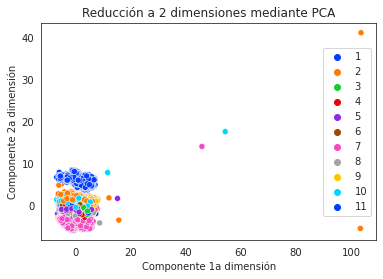
\includegraphics[width=0.6\textwidth]{images/repre_class}
		\caption{Visualizamos reducción 2-dimensional de los vectores de características (realizada mediante PCA)}
	\end{figure}
	
	Con las 2 componentes principales no se observa separabilidad de las clases. Desde luego trabajaremos con bastantes más dimensiones.
	\fi
	%Faltan por definir la clase de funciones hipótesis a usar y el algoritmo de aprendizaje.\\
	\iffalse
	Veamos una visualización del dataset $\mathcal{D}$ proporcionado 
	\begin{figure}[H]
		\centering
		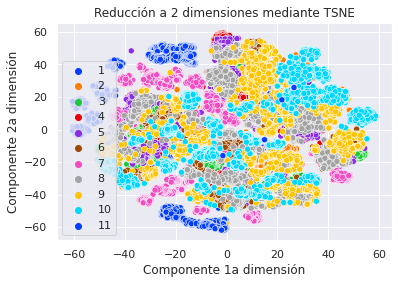
\includegraphics[width=0.8\textwidth]{images/class_tsne}
		\caption{Visualizamos reducción 2-dimensional de los vectores de características (realizada mediante t-SNE)}
	\end{figure}
	Teniendo en cuenta las 48 características no apreciamos ningún tipo de agrupamiento por clase al realizar la reducción de dimensionalidad.
	
	
	¿Se cumplirá que nuestra muestra es i.i.d.? Hay que comprobarlo pues es una de nuestras hipótesis. Para ello intentaremos ver correlaciones lineales mostrando, mediante mapa de calor, la matriz de coeficientes de correlación de Pearson:
	\begin{figure}[H]
		\centering
		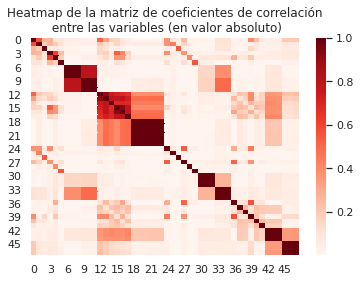
\includegraphics[width=0.57\textwidth]{images/corr_matrix_heatmap}
		\caption{Heatmap de la matriz de coeficientes de correlación entre la variables (en valor absoluto)}
	\end{figure}
	
	Se puede observar cierta correlación, basta ver las zonas rojas fuera de la diagonal (obivamente tenemos diagonal de 1s pues cada variable está determinada por sí misma), desde luego intentaremos que nuestra hipótesis de muestra i.i.d se cumpla, para ello intentaremos reducir esta correlación en la parte de preprocesamiento de datos.
	\fi
	\subsection{Clases de funciones a usar.}
	Realizaremos una transformación de segundo orden polinomial a los vectores de características, pues aumenta la flexibilidad de nuestra frontera de decisión. Para no aumentar en exceso la complejidad de la clase de funciones (mayor dimensión $\Rightarrow$ mayor complejidad $\Rightarrow$ mayor cota de error de generalización) reduciremos previamente la dimensionalidad de nuestros vectores de características (ver parte de preprocesado). No utilizamos transformación polinómica de mayor orden pues cuanto mayor sea la longitud de los vectores de características mayores posibilidades de disminuir el error en la muestra pero mayores posiblidades de aumentar error en la población (sobreajuste); a parte de incrementar el coste computacional.
	
	Por lo que, como hemos comentado, aplicaremos a  $\mathcal{X}$ la transformación $\Phi_2$, que genera combinaciones polinómicas de grado menor o igual a 2 de las características $$\Phi_2(\mathbf{x})=(1,x_1,\ldots, x_{\hat d},\underbrace{x_1x_2,\ldots ,x_1x_{\hat d},x_2x_3,\ldots ,x_2x_{\hat d},  \ldots
	 x_{\hat d-1}x_{\hat d}}_{\text{combinaciones } x_ix_j \text{ con } i<j,\ \  i,j\in \{1,\ldots , \hat d\}}, x_1^2,\ldots x_{\hat d}^2)^T$$
	%Realmente no podemos saber a priori cual es la mejor transformación que podemos hacer, debemos elegir una
	\textit{Nota:} aquí $\hat d< d=48$ pues no utilizaremos todas las características. Podemos ver que $\Phi_2(\mathbf{x})$ tiene $1+\hat d  + (\sum_{i=1}^{\hat d-1} \hat d -i) + \hat d  = 1 + 2\hat d + (\hat d -1)\hat d - \frac{(\hat d -1)\hat d}{2}=1+2\hat d + \frac{(\hat d -1)\hat d}{2}$ componentes\\
	
	Dentro de nuestros modelos utilizaremos enfoque probabilístico y determinístico. A continuación se exponen dos técnicas de minimización ya conocidas para enfoque probabilístico y determinístico respectivamente, junto con la clase de funciones hipótesis en cada caso. \\
	\textit{Nota:} para \texttt{RidgeClassifier} se busca solución analítica de la transformación de nuestro problema de clasificación a uno de regresión, y tendremos $\mathcal{H}:=\{h_w\colon \R^{2\hat d + \frac{(\hat d -1)\hat d}{2}+1}\to \R \ : \ h_w(\Phi_2(\mathbf{x}))=w^T\Phi_2(\mathbf{x}), \ w\in \R^{2\hat d + \frac{(\hat d -1)\hat d}{2}+1}\}$\\
	
	\textbf{Regresión Logística multiclase (One-vs-Rest):} $\quad \quad \quad \quad \quad \quad \quad \quad \quad \quad \quad \quad \quad \quad \quad \quad \quad  $ %(\texttt{SGDClassifier})
	
	Nuestra primera elección es utilizar Regresión Logística multiclase pues en situaciones reales tiene más sentido pensar situaciones probabilísticas que en funciones deterministas. Además la función de error será fácilmente minimizable mediante Gradiente Descendente Estocástico. Asignaremos cada vector de características a la clase que se estime más probable.\\
	
	Si 
	\begin{itemize}
	\item Tomamos como función objetivo $f\colon \mathcal{X} \to [0,1]^{11}$ con $f(\mathbf{x})=(P(y=1|\mathbf{x}),\ldots, P(y=11|\mathbf{x}))^T$ la función que asigna a cada vector de características el vector de probabilidades de pertenecer a cada clase 
	\item Denotamos con $d$ a $2\hat d + \frac{(\hat d -1)\hat d}{2}$
	\item Denotamos con $w_i$, $i=1,\ldots , K$, con $K=11$, el hiperplano que separa la clase $i$ del resto
	\end{itemize}
	tenemos la clase de funciones
	%$$\mathcal{H}:=\{h_{w_1,\ldots w_K} \colon \R^{d+1} \to \R^K \ : \ h_{w_1,\ldots w_K} (x)=(\sigma(w_1^T x), \ldots, \sigma(w_K^T x)),\ w_1,\ldots w_K \in \R^{d+1}\}$$
	%$$\mathcal{H}:=\{h_{w_1,\ldots w_K} \colon \R^{d+1} \to \R^K \ : \ h_{w_1,\ldots w_K} (\Phi_2(x))=Softmax((w_1^T \Phi_2(x), \ldots, w_K^T \Phi_2(x))^T),\ w_1,\ldots w_K \in \R^{d+1}\}=$$
	\begin{equation*}
\begin{aligned}
\mathcal{H}:= & \Big\{h_{w_1,\ldots w_K} \colon \R^{d+1} \to \R^K \ : \\
      & h_{w_1,\ldots w_K} (\Phi_2(x))=Softmax(\ (w_1^T \Phi_2(x), \ldots, w_K^T \Phi_2(x))^T \ ),\ w_1,\ldots w_K \in \R^{d+1}\Big\}
      \end{aligned}
\end{equation*}
	esto es
      \begin{equation*}
\begin{aligned}
      \mathcal{H}:=& \Big\{h_{w_1,\ldots w_K} \colon \R^{d+1} \to \R^K \ :\\
      & h_{w_1,\ldots w_K} (\Phi_2(x))=\frac{1}{\sum_{k=1}^K e^{w_k^T\Phi_2(x)}}(e^{w_1^T \Phi_2(x)}, \ldots, e^{w_K^T \Phi_2(x)})^T,\ w_1,\ldots w_K \in \R^{d+1}\Big\}
\end{aligned}
\end{equation*}
	%$$=\{h_{w_1,\ldots w_K} \colon \R^{d+1} \to \R^K \ : \ h_{w_1,\ldots w_K} (\Phi_2(x))=\frac{1}{\sum_{k=1}^K e^{w_k^T\Phi_2(x)}}(e^{w_1^T \Phi_2(x)}, \ldots, e^{w_K^T \Phi_2(x)})^T,\ w_1,\ldots w_K \in \R^{d+1}\}$$
	
	
	El error dentro de la muestra (máxima verosimilitud) es
	$$E_{in}(w_1,\ldots,w_K):=-\ln L(Y|w_1,\ldots ,w_K)=-\sum_{n=1}^N \sum_{k=1}^K y_{nk} \ln \sigma(w_k^T x_n)$$
	donde $\sigma$ es la función logística (sigmoide), $\sigma\colon \R \to [0,1]$, $\sigma(x)=\frac{1}{1+e^{-x}}=\frac{e^x}{e^x+1}$\\
	Vemos que
	$$\nabla_{w_j} E_{in}(w_1,\ldots,w_K)=\sum_{n=1}^N (\sigma(w_j^T x_n)-y_{nj}) x_n$$
	Utilizaremos SGD para minimizar (técnica ya explicada en el segundo aparatado del problema de regresión). Una vez acabada la optimización, obtendremos los $w_1,\ldots ,w_K$ que minimizan $E_{in}$. %Para asignar cada $x\in \mathcal{X}$ a una clase concreta se seguirá el criterio Softmax.
	 Asignaremos entonces cada $x$ a la clase más probable, es decir a la clase $j\in \{1,\ldots,K\}$ donde
	 $$j= \arg max_{j\in \{1,\ldots, K\}} \  \frac{exp(w_j^Tx)}{\sum_{k=1}^K exp(w_k^Tx)}$$
	%$$P(C_j |x)=\max_{k\in \{1,\ldots, K\}} P(C_k|x)= \max_{k\in \{1,\ldots, K\}} \frac{exp(w_jx)}{\sum_k exp(w_kx)}, \quad j=1,\ldots ,K$$
	
	\textbf{PLA-Pocket:} $\quad \quad \quad \quad \quad \quad \quad \quad \quad \quad \quad \quad \quad \quad \quad \quad \quad \quad \quad \quad \quad \quad \quad \quad \quad \quad \quad \quad  \quad $ %(\texttt{Perceptron})
	
	Recordamos que el \textit{Algoritmo de Aprendizaje Perceptron} es caso particular del algoritmo \textit{Gradiente Descendente Estocástico} para tamaño minibatch 1 y tasa de aprendizaje 1 para la función $error(w^T x_n, y_n)=\max \{0, -y_n w^T x_n\}$, las funciones hipótesis tiene la forma $h_w(x)=sign(w^Tx)$ donde $x$ tiene 1 en la primera componente.
    La regla de adapación del algoritmo es 
		$$\begin{cases}
		w_{updated} = w_{current} +y_ix_i & sign(w^Tx_i) \neq y_i\\
		w_{updated} = w_{current} & sign(w^Tx_i) = y_i
		\end{cases} \quad \quad (*)$$
		es decir, teniendo un dataset $\mathcal{D}$ de tamaño $N$, $\mathcal{D}=\{(x_1,y_1),\ldots,(x_N,y_N)\}$, lo que hacemos es recorrerlo con $i=1,\ldots, N$ y actuar conforme (*) para cada $i$. Por lo que, si $x_i$ no está bien clasificado, entonces actualizamos el vector de pesos actual, $w$, en la dirección correcta; si está bien casificado no se hace nada. Estos recorridos del dataset siguiendo este criterio los repetimos hasta que se consiga un recorrido completo del dataset en el que no haya ningún punto mal clasificado.\\
		\textit{Nota:} si la muestra no es separable el algoritmo no llegará a clasificar correctamente toda la muestra, en este caso debe añadirse otra condición de parada, número máximo de épocas por ejemplo.\\
		
	PLA-Pocket equivale a PLA con dos distinciones: (1) no hay restricción de seguir mientras haya puntos mal clasificados, pues la idea es utilizarlo en muestras no separables, y (2) iremos anotando la mejor solución obtenida hasta el momento, la que proporcione menor error en la muestra. Al completar las épocas máximas indicadas se devolverá el vector de pesos óptimo.\\
	En nuestro caso, de nuevo denotando con $d$ a $2\hat d + \frac{(\hat d -1)\hat d}{2}$, tenemos la clase de funciones
	$$\mathcal{H}:=\{h_w\colon \R^{d+1} \to \R \ : \ h_w(\Phi_2(x)) = sign(w^T\Phi_2(x)), \ w \in \R^{d+1}\}$$
	La función de error a minimizar es 
	$$E_{in}(h_w):= \frac{1}{N} \sum_{n=1}^N [[h_w(\Phi_2(x))\neq y_n]]$$
	
	\textbf{Modelo por regresión:}
	
	El último de nuestros modelos consiste en transformar el problema de clasificiación a uno de regresión y tendremos $\mathcal{H}:=\{h_w\colon \R^{2\hat d + \frac{(\hat d -1)\hat d}{2}+1}\to \R \ : \ h_w(\Phi_2(\mathbf{x}))=w^T\Phi_2(\mathbf{x}), \ w\in \R^{2\hat d + \frac{(\hat d -1)\hat d}{2}+1}\}$, $E_{in}(w)=\frac{1}{N}\norm{Xw-y}^2$
	
	\subsection{Hipótesis finales que se usarán.}
	En el preprocesado: (1) se eliminan características con coeficiente de correlación lineal en valor absoluto mayor a 0.95, (2) se eliminan las características con varianza 0, (3) se seleccionan las 20 características con mejor resultado por test ANOVA, (4) se realiza transformación polinomial de segundo orden a cada vector de características, (5) se normalizan las características (media 0 y varianza 1).
	
	La métrica a valorar es accuracy. Evaluaremos desempeño de métodos \texttt{Perceptron} (PLA-Pocket), \texttt{OneVsRestClassifier} junto con \texttt{SGDClassifier} (Regresión Logística multiclase One-vs-Rest (SGD)) y \texttt{RidgeClassifier} (solución analítica de regresión por SVD a la transformación del problema de clasificación a uno de regresión). Para cada uno evaluaremos mediante 5-fold cross validation los parámetros de regularización $0.00001$, $0.001$ y $0.1$ para regularización Ridge
	\subsection{Generación de conjuntos training y test.}
	Hay un compromiso en la selección del tamaño de entrenamiento y test: el tamaño de la muestra de entrenamiento determina el número de instancias que tendremos para entrenar el modelo y por tanto para minimizar $E_{in}$, y el  tamaño del conjunto de test condicionará la estimación, $E_{test}$, de $E_{out}$ que obtengamos. Evitaremos proporciones extremas para tamaño de test. Suele ser habitual reservar un 20\% de las instancias para test, y eso hemos hecho. De las 58509 instancias tendremos 11702 para test, el resto para training y validación cruzada. La división en training y test se ha hecho conservando la proporción de clases, esto se hace para que tanto training como test sean los más representativos posibles de la distribución de la que provienen.
	
	Utilizaremos $k$-fold cross validation con $k=5$ para la selección de modelos. Esta técnica es derivada de \textit{Leave-one-out}, la cual nos proporciona una estrategia para abordar la problemática o compromiso de elección del tamaño de conjunto de validación, $K$, esta es: $E_{out}(g)\approx E_{out}(g^-)$ cuando $K$ pequeño y $E_{out}(g^-)\approx E_{val}(g^-)$ cuando $K$ grande. %Lo ideal sería utilizar $N$-fold cross validation que equivale a \textit{Leave-one-out}, pero tiene un alto coste computacional.
	
	 La técnica $k$-fold cross validation consiste en dividir la muestra de entrenamiento en $k$ particiones, cada una de tamaño aproximado $\frac{N}{k}$, e ir iterando sobre ellas eligiendo cada vez una partición para actuar como conjunto de validación y entrenando sobre el resto de la muestra el modelo; una vez iteradas sobre todas las particiones se toma la media de errores obtenidos y ese es el error de validación cruzada $E_{cv}\iffalse=\frac{1}{N}\sum_{i=1}^N E_{val}(g_i^-)\fi$ que es un buen estimador de $E_{out}$ cuando $k$ es grande, cuanto menor sea $k$ peor será la estimación de $E_{out}$. Se elige el modelo con menor $E_{cv}$
	 
	  Se podría tomar $k=N$ pero esto implica un alto coste computacional; es por esto que se elige $k<< N$, en nuestro caso $k=5$ (es habitual $5\leq k\leq 10$)
	\subsection{Detalles del preprocesado de datos.}
	Pasos realizados:
	\begin{enumerate}
		\item Se eliminan las características que tienen valor absoluto de coeficiente de correlación lineal mayor a 0.95 con otra característica. %Se puede decir que éstas no nos aportan información nueva.
		
		Esto se hace porque se observó la matriz de coeficientes de correlación lineal en valores absolutos
		\begin{figure}[H]
		\centering
		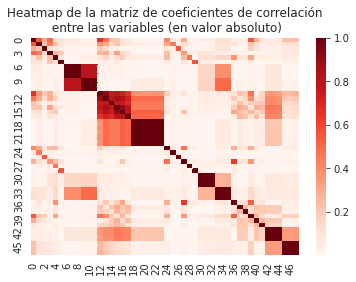
\includegraphics[width=0.5\textwidth]{images/corr_matrix}
		\caption{Matriz de coeficientes de correlación en valor absoluto}
		\end{figure}
		Las características $7, 8, 10, 11, 19, 20, 21, 22, 23, 31, 32, 34, 35, 43, 44, 46, 47$ tenían valores de coeficiente de correlación mayor a 0.95 en la matriz. Se puede decir que estas características no nos aportan información nueva, además aumentan la dimensionalidad y por tanto empeoran la cota de error de generalización. Se decide eliminarlas y reducir así la complejidad de la clase de funciones. Tras eliminarlas se obtiene
		\begin{figure}[H]
		\centering
		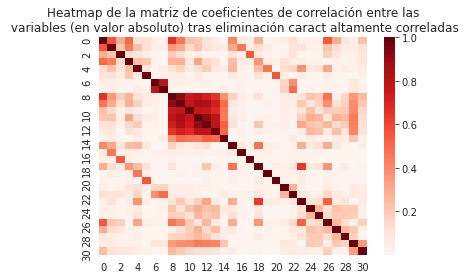
\includegraphics[width=0.62\textwidth]{images/corr_matrix_post}
		\caption{Matriz de coeficientes de correlación en valor absoluto tras la eliminación de características altamente correladas linealmente}
		\end{figure}
		una matriz de menor dimensión y con menor apreciación de zonas correspondientes a alta correlación (excepto en diagonal donde tenemos coeficientes de correlación 1 pues es la correlación de cada característica consigo misma).
		\item Eliminamos las características con varianza 0 si las hubiese, no aportan ninguna información y además es necesario eliminarlas para después normalizar.
		%\item Normalizamos las características, no normalizarlas degrada el desempeño de la regularización.
		%\item Una vez normalizadas y teniendo ????
		\item Seleccionamos las 20 características con mejor resultado (posible mayor ``impacto'' en etiquetado) en test ANOVA, el número elegido es totalmente arbitrario, se decidió elegir una cantidad algo mayor a la mitad de las características; suficiente para no quedarnos con pocas características y perder información, pero tampoco excesiva como para no poder manejar el coste computacional del aumento de dimensionalidad tras la transformación polinómica (con 20 características ya aumentaremos hasta 231 características).\\
		La elección de este método ha sido arbitraria, se podría haber elegido cualquier otro método para reducir la dimensionalidad y complejidad de la clase de funciones.
		\item Realizamos transformación polinomial de segundo orden a cada característica para aumentar así la flexibilidad de la frontera de decisión nuestro modelo.
		\item Normalizamos las características (tendrán media 0 y varianza 1), no normalizar puede degradar el desempeño de algoritmos como Perceptron y Regresión Logística mediante SGD. También deben estar normalizadas de cara a que nuestra regularización actúe correctamente. Normalizamos para evitar estas problemáticas y que todas las características ``sean valoradas en la misma magnitud''. %Volvemos a normalizar las características (que dos variables aleatorias tengan distribución normal no implica que su producto tenga distribución normal)
	\end{enumerate}
	\subsection{Métrica de error a usar.}
	Visualizaremos el número de vectores de características de la realización muestral pertenecientes a cada clase, esto nos mostrará si hay clases desbalanceadas y qué métrica necesitamos utilizar.
	\begin{figure}[H]
		\centering
		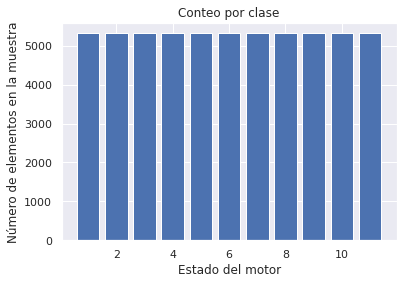
\includegraphics[width=0.51\textwidth]{images/conteo_por_clase}
		\caption{Número de elementos por estado de motor}
	\end{figure}
	
	Como podemos ver las clases están balanceadas, de hecho el número de elementos por clase no cambia, tenemos 5319 elementos en todas las clases. Como no tenemos clases desbalanceadas utilizaremos la métrica $accuracy$ que no es más que la proporción de predicciones de clase correctas.
	%$$accuracy:= \frac{TP + TN}{P + N}$$
	%nos da la proporción de predicciones correctas (tanto positivas como negativas). Aquí \textit{TP} denota el número de predicciones positivas correctas, \textit{TN} el número de predicciones negativas correctas, \textit{P} el número verdadero de puntos con etiqueta positiva y \textit{N} el número verdadero de puntos con etiqueta negativa.
	%No necesitamos fijarnos en ninguna métrica especial, basta con minimizar el error en la muestra, conseguir $g$ con el mayor accuracy.\\
	
	
	\subsection{Parámetros usados y tipo de regularización elegida.}
	La regularización nos ayudará a evitar sobreajuste, sobretodo después de la transformación polinómica que hemos realizado. Con la regularización se aumentará ligeramente el sesgo para decrementar significativamente la varianza. Utilizaremos regularización Ridge, ahora tendremos error aumentado 
	$$E_{aug}(\mathbf{w})=E_{in}(\mathbf{w})+\lambda \norm{\mathbf{w}}_2^2 = E_{in}(\mathbf{w})+\lambda \mathbf{w}^T\mathbf{w}$$
	donde $\lambda \geq 0$ es el parámetro de regularización. Este tipo de regularización penaliza coeficientes de $\mathbf{w}$ grandes. Otro tipo de regularización muy conocida es regularización Lasso (utiliza norma $\norm{\cdot}_1$ en lugar de norma $\norm{\cdot}_2$), ésta sin embargo tiende a hacer coeficientes de $\mathbf{w}$ a 0, es buena para selección de características. En nuestro caso todas las características son de la misma naturaleza (señales eléctricas) y confiamos en la selección de características relevantes que hicimos, es por esto que preferimos regularización Ridge antes que Lasso.\\
	%Dos tipos de regularización conocidas son la regularización $l_1$ o Lasso y la regularización $l_2$ o Ridge. La primera es buena para selección de variables, cuando se minimiza hace varios coeficientes 0. La segunda suele dar valores bajos de los coeficientes, penaliza coeficientes altos.
	
	%En nuestro caso se elige regularización Ridge, ya hemos hecho previamente una selección de variables.\\
	
	En Regresión Logística hemos utilizado la función \texttt{OneVsRestClassifier} junto con \texttt{SGDClassifier}, sigue el criterio one vs rest que es el explicado la sección \textit{Clase de funciones a usar} y el que utilizaremos. \texttt{SGDClassifier} utiliza tamaño de minibatch 1. Es interesante notar que la función de error junto con el término de regularización Ridge es convexa; pierde relevancia el uso de minibatches o punto de inicio al no tener óptimos locales. Se podría utilizar Gradiente Descendente sin ningún problema. Aún así, dado que \texttt{sklearn} nos proporciona método para la versión estocástica, y que realmente ganamos eficiencia computacional al calcular gradiente en un solo punto, y el ruido que supone computar el gradiente en un solo punto termina promediándose en número alto de iteraciones; se decide utilizar la versión que nos facilita \texttt{sklearn}. El learning rate se ha elegido adaptativo, cuando no se esté mejorando en el criterio de tolerancia tras \texttt{n\_iter\_no\_change} épocas, entonces actualizamos la tasa de aprendizaje mediante $learning\_rate =\frac{learning\_rate}{5}$, vamos disminuyendo conforme nos acercamos al mínimo para prevenir oscilación. Se ha elegido learning rate inicial algo elevado puesto que es adaptativo y una tolerancia arbitraria \texttt{tol} 0.001 a la que daremos hasta 5 épocas para que se halla disminuido en \texttt{tol} el error. El algoritmo parará si tenemos learning rate menor a 1e-6 o por iteraciones máximas. Se adjunta código con comentarios del resto de parámetros:
	\begin{lstlisting}[language=Python, caption= Par\'ametros usados en SGDClassifier, inputencoding=latin1]
  {"model": [OneVsRestClassifier(SGDClassifier(loss = 'log', # función de pérdida de regresión logística
                                 penalty = 'l2', # utilizaremos regularización l2
                                 # alpha  constante del término de regularización (probaremos distintos valores mediante 5-fold cross validation)
                                 fit_intercept = True, # añadimos sesgo o intercept pues nuestra matriz aún no tiene columna de 1s 
                                 max_iter = 80, # Número máximo de iteraciones arbitrario
                                 tol = 0.001, # Tolerancia para criterio de parada por tolerancia (parar si loss > best_loss - tol tras n_iter_no_change épocas seguidas)
                                             # el criterio valora si el error es no mejora en 0.001 el mejor error hasta el momento. En nuestro caso esta condición por tolerancia se usará para learning_rate adaptativo
                                 shuffle = True, # mezclamos después de cada época
                                 n_jobs = -1, # máxima paralelización posible en ejecución
                                 random_state = 1, # para tener reproducibilidad de los resultados
                                 learning_rate = 'adaptive', # si no se mejora resultado por criterio tolerancia (loss > best_loss - tol) tras n_iter_no_change épocas seguidas, entonces cambiamos learning rate por (learning rate)/5
                                                             # queremos evitar oscilación
                                 eta0 = 0.05, # learning rate inicial arbitrario
                                 early_stopping = False, # False pues no queremos reservar más datos para validación
                                 n_iter_no_change = 5, # cada 5 épocas sin mejora en crit. tolerancia se realizará la adaptación del learning rate (learning_rate='adaptive')
                                 class_weight = None, # se iterpreta que todas las clases tienen peso 1, que es el caso
                                 average = False, # no nos interesa obtener media de pesos
                                 verbose = 0, # no nos interesan mensajes 
                                 warm_start = False, # no reutilizamos ninguna solución anterior durante la validación cruzada
                                 l1_ratio = 0 # 0 corresponde a l2 penalty, no se usará pues solo se usa si learning_rate = 'elasticnet'
                                 ), n_jobs= -1)], # máxima paralelización posible
         "model__estimator__alpha": [0.00001, 0.001, 0.1]}, # probamos valores de regularización arbitrarios dentro de los recomendados

	\end{lstlisting}
	
	Para PLA-Pocket se utiliza la función \texttt{Perceptron}, se adjunta código con comentarios sobre los parámetros elegidos:
	\begin{lstlisting}[language=Python, caption= Par\'ametros usados en Perceptron, inputencoding=latin1]
  {"model": [Perceptron(penalty = 'l2', # utilizaremos regularización l2
                            # alpha  constante del término de regularización (probaremos distintos valores mediante 5-fold cross validation)
                            # l1_ratio solo si usa si penalty='elasticnet' que no es el caso
                            fit_intercept = True, # añadimos sesgo o intercept pues nuestra matriz aún no tiene columna de 1s 
                            max_iter = 80, # Número máximo de iteraciones arbitrario
                            #tol  por defecto, arbritraria, si tenemos loss > previous_loss - tol paramos
                            shuffle = False, # no mezclamos la muestra tras cada época
                            eta0 = 1, # =1 para no multiplicar las actualizaciones, no las alteramos
                            n_jobs = -1, # máxima paralelización posible en ejecución
                            random_state = 1, # para tener reproducibilidad de los resultados
                            early_stopping = False, # no nos interesa reservar más datos para validación (nuestro único criterio de parada serán las iteraciones)
                            # validation_fraction no será usado pues early_stopping = False
                            # n_iter_no_change no será usado pues early_stopping = False
                            class_weight = None, # None se interpreta como que todas las clases tienen peso 1, que es el caso
                            warm_start = False # no reutilizamos ninguna solución anterior durante la validación cruzada
                            )], 
         "model__alpha": [0.00001, 0.001, 0.1]}, # probamos valores de regularización arbitrarios dentro de los recomendados
	\end{lstlisting}
	
	Por último utilizaremos \texttt{RidgeClassifier}, que transforma el problema de clasificación en uno de regresión y resuelve el de regresión (en nuestro caso lo resolveremos de forma analítica mediante descomposición en valores singulares), a pesar de esto no suele dar malos resultados. Adjuntamos código con comentarios sobre los parámetros elegidos:
	\begin{lstlisting}[language=Python, caption= Par\'ametros usados en \texttt{RidgeClassifier}, inputencoding=latin1]
  {"model": [RidgeClassifier(# alpha  constante del término de regularización (probaremos distintos valores mediante 5-fold cross validation)
                        fit_intercept=True, # añadimos sesgo o intercept pues nuestra matriz aún no tiene columna de 1s 
                        normalize=False, # no nos interesa normalizar, ya lo hicimos en preprocesado
                        copy_X=True, # no nos interesa sobreescribir X
                        max_iter=None, # None pues no usaremos método iterativo
                        tol=0.001, # precisión de la solución, lo dejamos por defecto, no nos importa pues utilizaremos solución analítica por SVD
                        class_weight=None, # None se interpreta como que todas las clases tienen peso 1, que es el caso
                        solver='svd', # resolveremos de forma analítica usando descomposición en valores singulares 
                        random_state=None)], # no nos hace falta para tener reproducibilidad de los resultados pues no se va a usar solver=sag o solver=saga. Obtendremos solución analítica
         "model__alpha": [0.00001, 0.001, 0.1]}, # probamos valores de regularización arbitrarios dentro de los recomendados
	\end{lstlisting}~\\
	
	\textit{Nota en general:} el número de iteraciones, \texttt{n\_iter\_no\_change} y tolerancia se han elegido de forma arbitraria y comprobando que hubiese convergencia. Estos parámetros se podrían haber añadido como parámetros a valorar y expandir nuestro número de modelos para validación cruzada, pero los tiempos de ejecución serían inabarcables.
	
	\subsection{Selección de la mejor hipótesis y $E_{out}$}
	Para la selección de la mejor hipótesis o modelo utilizaremos 5-fold cross validation, técnica ya explicada en la sección de \textit{Generación de conjuntos training y test}. Elegiremos como modelo ganador aquel con menor $E_{cv}$. El modelo ganador se entrenará finalmente sobre toda la muestra.
	
	Para hacer esto se ha utilizado \texttt{GridSearchCV}, función que nos permite entrenar el modelo ganador en toda muestra mediante \texttt{refit=True}, y nos facilita la visualización de resultados. La métrica considerada para elección del mejor modelo es el \textit{accuracy} (tenemos clases perfectamente balanceadas)
	
	Vamos a valorar distintos parámetros de regularización: tanto para Regresión Logística multiclase (\texttt{OneVsRestClassifier} con \texttt{SGDClassifier}) como para PLA-Pocket (\texttt{Perceptron}) y solución por regresión (\texttt{RidgeClassifier}) tendremos los parámetros de regularización $0.00001$, $0.001$ y $0.1$, por lo que en total tendremos 9 modelos para 5-fold cross validation (se podrían tener más modelos considerando otros parámetros, nos hemos limitado a los parámetros de regularización indicados)
	
	Nos referiremos a los modelos o hipótesis determinados en última instancia por \texttt{OneVsRestClassifier} con \texttt{SGDClassifier}, \texttt{Perceptron} y \texttt{RidgeClassifier} (junto sus parámetros) mediante $M_{RL}$, $M_{PLA-Pocket}$, $M_{Regre}$ respectivamente (representan todos los pasos realizados: preprocesado, clase de funciones elegida, parámetros...). Tendremos 9 modelos determinados finalmente por los parámetros de regularización: $$\{(M_{PLA-Pocket},\lambda),(M_{RL},\lambda), (M_{Regre},\lambda)\} \ \ \text{ con } \ \  \lambda \in \{0.00001, 0.001, 0.1\}$$
	
	Veamos los accuracies medios de cada modelo obtenidos por 5-fold cross validation
	%$(M_{PLA-Pocket},0.00001),\\ (M_{PLA-Pocket},0.0001), (M_{PLA-Pocket},0.1), (M_{RL},0.00001), (M_{RL},0.0001), (M_{RL},0.1)$
	\begin{table}[H]
	\begin{center}
	\begin{tabular}{|c|c|c|}
	\hline
	 Modelo & Accuracy medio 5-fold cross validation \\
	\hline \hline
	$(M_{RL},0.00001)$ & 0.94853335 \\ \hline
	$(M_{RL},0.001)$ & 0.89749403 \\ \hline
	$(M_{RL},0.1)$ & 0.69619929 \\ \hline
	$(M_{PLA-Pocket},0.00001)$ & 0.7828322 \\ \hline
	$(M_{PLA-Pocket},0.001)$ & 0.4353621 \\ \hline
	$(M_{PLA-Pocket},0.1)$ & 0.19939233 \\ \hline
	$(M_{Regre},0.00001)$ & 0.78894203 \\ \hline
	$(M_{Regre},0.001)$ & 0.7891984 \\ \hline
	$(M_{Regre},0.1)$ & 0.78590836 \\ \hline
	\end{tabular}
	\caption{Accuracies medios por 5-fold cross validation de cada modelo}
	\label{tabla:sencilla}
	\end{center}
	\end{table}
	Nuestro mejor modelo con accuracy medio por 5-fold cross validation 0.94853335 es $(M_{RL},0.00001)$, podemos ver que valores mayores de regularización nos dan peores resultados (menor accuracy). Desde luego es destacable la gran mejora en accuracy obtenida con un pequeño valor de regularización; al aumentar valores de $\lambda$ estamos imponiendo restricción cada vez más fuerte y el modelo deja de ajustar bien como podemos observar, para $(M_{RL},\lambda)$ con $\lambda=0.1$ obtenemos accuracy 0.69619929, bastante peor. 
	
	Para $M_{PLA-Pocket}$ el máximo accuracy también se obtiene con el menor valor de regularización, aunque se obtiene accuracy 0.7828322, considerablemente peor que 0.94853335, al igual que antes valores mayores de $\lambda$ empeoran los resultados, en este caso aún más notable: $(M_{PLA-Pocket},\lambda)$ con $\lambda =0.1$ nos da accuracy 0.19939233
	
	 Finalmente podemos observar el mismo fenómeno de peores resultados al aumentar el término de regularización  en $M_{Regre}$, y sorprendentemente vemos que hemos obtenido, con cualquier término de regularización, accuracies ligeramente superiores al mejor obtenido por $M_{PLA-Pocket}$, vemos que, a pesar de transformar el problema de clasificación a uno de regresión y utilizar una función de pérdida de error cuadrático medio, obtenemos buenos resultados.\\
	
	Entrenamos nuestro modelo ganador $(M_{RL},0.00001)$ con todos los datos de entrenamiento. Al utilizar todos los datos de entrenamiento tenemos la ventaja de tener un tamaño de entrenamiento mayor (en 5-fold cross validation no utilizábamos $N$ instancias, siempre reservábamos una de las 5 particiones para validar). Entrenando sobre toda la muestra de entrenamiento se espera ahora obtener un ``mejor regresor''.
	
	 Utilizaremos nuestro conjunto de test que guardamos desde el principio para estimar el error de generalización, estimaremos $E_{out}$ mediante $E_{test}$. Procediendo así, y teniendo en cuenta que estamos valorando mediante la métrica accuracy, estimamos error, de nuestro mejor modelo $(M_{RL},0.00001)$, fuera de la muestra: 1-0.94966672=0.05033328; estimación ligeramente más optimista que la que obteníamos en validación cruzada ($0.94966672>0.94853335$), lo cual va en consonancia con el resultado teórico $E_{out}(g) \leq E_{cv}$ (va en consonancia en el sentido de que $E_{out}(g)\approx E_{test}(g)\leq E_{cv}$), que nos viene a decir que el error de validación cruzada, $E_{cv}$, nos da una estimación pesimista del error de generalización.
	%$E_{out}$ no se puede conocer solo estimar. Recordamos que el error $E_{cv}$  es buen estimador de $E_{out}$ ($E_{cv}$ es estimador insesgado de $\overline{E}_{out}(N-1)$; además $E_{out}(g) \leq E_{cv}$\iffalse , aunque trabajaremos con estimaciones y nos limitamos a unos datos por lo que no siempre se tiene que cumplir\fi ). Teniendo en cuenta que estamos valorando mediante la métrica accuracy, estimamos, de nuestro mejor modelo, $(M_{RL},0.00001)$, error fuera de la muestra 1-0.9487897=0.0512103
	\subsection{$E_{out}$ para la mejor hipótesis usando todos los datos para entrenar.}
	Ahora utilizamos todos los datos disponibles para entrenar nuestro mejor modelo, esto nos dará un mejor ajuste. Para estimar $E_{out}$ ya no disponemos de conjunto de test. Lo que se hará es hacer uso de la cota pesimista de que nos proporciona $E_{cv}$, tendremos una cota superior de $E_{out}(g)$. La cota será más ajustada cuanto mayor sea $k$ en $k$-fold cross validation, idealmente $k=N$ (Leave-one-out); de nuevo, por el alto coste computacional que esto supondría, nos conformaremos con $k=20$\\
	Procediendo así, y teniendo en cuenta que estamos valorando mediente la métrica accuracy, estimamos $E_{out}(g)\leq 1-0.9500247413405309=0.04997525865946906$. Es destacable que al estar usando todos los datos disponibles para entrenar estamos obteniendo un ``mejor clasificador'', estamos obteniendo como cota pesimista de $E_{out}$ un valor menor que la estimación de $E_{out}$ por $E_{test}$ cuando solo usábamos el conjunto de training para entrenar (que a su vez era menor que el error de validación cruzada).
	%Procediendo así, y teniendo en cuenta que estamos valorando mediente la métrica accuracy, estimamos $E_{out}(g)\leq 1-0.9500247413405309=0.04997525865946906$. Es destacable que al estar usando todos los datos disponibles para entrenar estamos obteniendo un ``mejor clasificador'', estamos obteniendo como cota pesimista de $E_{out}$ un valor menor que: $E_{cv}$ y estimación de $E_{out}$ por $E_{test}$ cuando solo usábamos el conjunto de training para entrenar.
	%Al utilizar todos los datos tenemos la ventaja de tener un tamaño de entrenamiento mayor (en 5-fold cross validation no utilizábamos $N$ instancias, siempre reservábamos una de las 5 particiones partición para validar). Entrenando sobre toda la muestra de entrenamiento se espera ahora obtener un ``mejor clasificador''. 
	
	%En este caso, para estimar $E_{out}$ utilizaremos el conjunto de test que guardamos desde el principio, calcularemos $E_{test}$. Procediendo así, estimamos error fuera de la muestra 1-0.95009400=0.049906 fuera de la muestra, estimación algo más optimista que la que obteníamos en validación cruzada (se corresponde a un menor error, va en concordancia la desigualdad anteriormente mencionada $E_{out}(g) \leq E_{cv}$).
	
	
\end{document}
	

